\documentclass{article}

\usepackage{graphicx}
\usepackage{mathtools}
\usepackage{harpoon}
\usepackage{float}
\usepackage[margin=1.0in]{geometry}

\title{Tran{}sformations in Three Dimensional Space}
\date{2019}
\author{Aaron Thompson}

\begin{document}

	\begin{titlepage}
		\pagenumbering{gobble}
		
		\maketitle
	
		\newpage
	
		\tableofcontents
	\end{titlepage}

	\pagenumbering{arabic}

	\newpage

	\section{Introduction}
	Much of mathematics is performed in only one or two dimensions. When considering and manipulating objects in three dimensional space, an additional layer of complexity is added. Rather than only having to consider the x-axis and y-axis, the position of a point in the z-axis also has to be considered. My interest in 3D math began to explore 3D graphics. I have been interested in graphics programming for a long time, but distanced myself from three dimensional problems. As I began to look into 3D graphics recently, I saw that the math involved was very unique and challenging. Because of this, I chose to look into it more deeply for my exploration. \par

	Three-dimensional points can be represented as 3-element vectors, where the top value is the x-coordinate, the middle value is the y-coordinate, and bottom value is the z-coordinate. While this is sufficient for modeling the position of a coordinate, a lot of operations required to translate this position vector will end up requiring a fourth element. This is the "w-coordinate" of the point. For the purposes of most operations done in this document, the w-coordinate of all position vectors will remain 1, and the w-coordinate of all other vectors will be 0. The need for this will be shown in future sections and examples.
	
	\subsection{Matrices}

	Some three dimensional translations require the use of matrices to be performed. A matrix is a mathematical object in which numbers are arranged into both columns and rows. They can be thought of as a collection of a different object we are familiar with in IB Math: The vector. For example, the $4 \times 4$ matrix that is commonly used in three dimensional math, can be thought of as a collection of 4 vectors, each with 4 elements. \par

	In order to be able to use matrices in the coming math, the basic operation of multiplication has to be defined. Matrix multiplication requires more steps that the simple multiplication of one number. There is a process that is required. \par

	Matrix multiplication is not commutative. The order in which different matrices are multiplied will affect what the result is, or might even make the multiplication impossible. In order for two matrices to be able to be multiplied, the width of the matrix on the left side of the multiplication must be equal to the height of the right matrix. The resultant matrix will have the dimensions of the height of the left matrix, and the width of the right matrix. In order to get each element of the resultant array, a dot product has to be taken. This is best illustrated using an example: \par

	% Use matrices with elements [x11, x12, x13, ...] and [y11, y12, y13, ...]. Use the dimensions from Mr Tubb's example for illustrative purposes.
	% Put a \times symbol between them and then write [r11, r12, r13, ...] for the resultant
	% After the figure, place the following text:
	\[
		\begin{bmatrix}
			x_{11} & x_{12} \\
			x_{21} & x_{22} \\
			x_{31} & x_{32}
		\end{bmatrix}
		\bullet
		\begin{bmatrix}
			y_{11} & y_{12} & y_{13} & y_{14} \\
			y_{21} & y_{22} & y_{23} & y_{24}
		\end{bmatrix}
		=
	\]
	\[
		\begin{bmatrix}
			x_{11} y_{11} + x_{12} y_{21} & x_{11} y_{12} + x_{12} y_{22} & x_{11} y_{13} + x_{12} y_{23} & x_{11} y_{14} + x_{12} y_{24} \\
			x_{21} y_{11} + x_{22} y_{21} & x_{21} y_{12} + x_{22} y_{22} & x_{21} y_{13} + x_{22} y_{23} & x_{21} y_{14} + x_{22} y_{24} \\
			x_{31} y_{11} + x_{32} y_{21} & x_{31} y_{12} + x_{32} y_{22} & x_{31} y_{13} + x_{32} y_{23} & x_{31} y_{14} + x_{32} y_{24}
		\end{bmatrix}
	\]

	In order to find the value of a given cell of the resultant matrix, the dot product is taken of the corresponding row of the left matrix, and the corresponding column of the right matrix. \par

	A special matrix is the identity matrix. Multiplying a matrix by an identity matrix of the same size will result in the same matrix. It looks like this: \par

	\[
		\begin{bmatrix}
			1 & 0 & 0 & 0 \\
			0 & 1 & 0 & 0 \\
			0 & 0 & 1 & 0 \\
			0 & 0 & 0 & 1
		\end{bmatrix}
	\]
	
	This matrix will act as the starting point for many of our transformations, because it represents the starting point of a transformation. It can then be manipulated purposefully to achieve what is needed.

	\section{Translation}

	Translation is a change in the position of a point. In a way, all other transformations are based on this. It is one of the most common operations in video games: Translating the player character to navigate the world, translating particles to create effects, and so on. A simple way to complete a translation is to add two vectors:
	\[
		\begin{pmatrix}
			x \\
			y \\
			z
		\end{pmatrix}
		+
		\begin{pmatrix}
			V_{x} \\
			V_{y} \\
			V_{z}
		\end{pmatrix}
		=
		\begin{pmatrix}
			x + V_{x} \\
			y + V_{y} \\
			z + V_{z}
		\end{pmatrix}
	\]
	\par
	Being able to complete these transformation with a matrix however, will allow us to combine them into a single mathematical object later on. This would be impossible, or at the least unwieldy, using vectors. \par
	There is no good way to complete this operation using a three-element vector and a matrix. However, if a 4th element is introduced into the vector with value 1, then the transformation is simple: \par
	\[
		\begin{bmatrix}
			1 & 0 & 0 & V_{x} \\
			0 & 1 & 0 & V_{y} \\
			0 & 0 & 1 & V_{z} \\
			0 & 0 & 0 & 1
		\end{bmatrix}
		\bullet
		\begin{pmatrix}
			x \\
			y \\
			z \\
			1
		\end{pmatrix}
		=
		\begin{pmatrix}
			x + V_{x} \\
			y + V_{y} \\
			z + V_{z} \\
			1
		\end{pmatrix}
	\]

	An identity matrix is used to preserve the ($x, y, z$) coordinates of the original point. Then, the elements of the translation vector are aligned in the rightmost column of the translation matrix. In this position, they are multiplied by the w-component, 1, when the dot product is taken. This means that coordinates and the translation remains unchanged, and they are simply added together.

	\subsection{Example}
	Consider a point \(p = \begin{psmallmatrix} -2 \\ 1 \\ 1 \\ 1 \end{psmallmatrix}\)
	to be transformed by direction vector \(v = \begin{psmallmatrix} 3 \\ -2 \\ -2 \end{psmallmatrix}\).
	The components of the direction vector go in to the transformation matrix in the respective positions to produce the following matrix for the translation: \par
	\[
		\begin{bmatrix}
			1 & 0 & 0 & 3 \\
			0 & 1 & 0 & -2 \\
			0 & 0 & 1 & -2 \\
			0 & 0 & 0 & 1
		\end{bmatrix}
	\]

	Multiplying this matrix by $p$ will yield the translated $p'$:
	\[
		\begin{bmatrix}
			1 & 0 & 0 & 3 \\
			0 & 1 & 0 & -2 \\
			0 & 0 & 1 & -2 \\
			0 & 0 & 0 & 1
		\end{bmatrix}
		\bullet
		\begin{pmatrix}
			-2 \\
			1 \\
			1 \\
			1
		\end{pmatrix}
		=
		\begin{pmatrix}
			-2 + 3 \\
			1 - 2 \\
			1 - 2 \\
			1
		\end{pmatrix}
		=
		\begin{pmatrix}
			1 \\
			-1 \\
			-1 \\
			1
		\end{pmatrix}
	\]

	\begin{figure}[H]
		\centering
		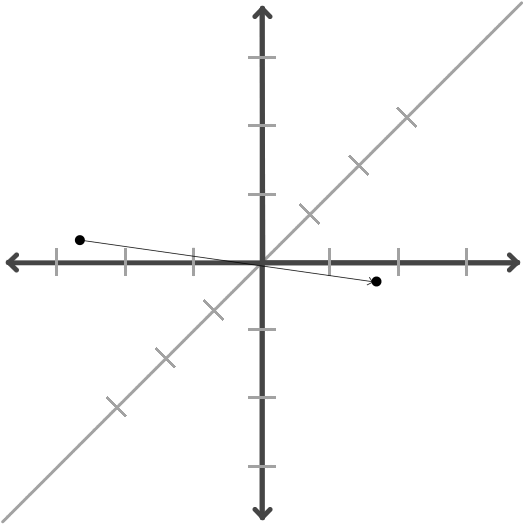
\includegraphics{img/translation.png}
		\caption{Visualization of translation described above.}
	\end{figure}

	\section{Scaling}

	Scaling expands all points away from the origin by some scale factor. Practically, this can be used to create the illusion of a 3-dimensional environment, by scaling objects with a larger z-value down, and scaling up object with a smaller z-value, as an example. Scaling could be achieved by multiplying all position vectors of a figure by the scale factor: \par

	\[
		c \cdot
		\begin{pmatrix}
			x \\
			y \\
			z \\
			1
		\end{pmatrix}
		=
		\begin{pmatrix}
			cx \\
			cy \\
			cz \\
			c
		\end{pmatrix}
	\]
	
	However, being able to complete this transformation with the use of a matrix can be useful when combining transformations. Furthermore, this causes the $w$ value of the vector to become a value other than 1, potentially interfering with operations performed in the future.\par

	In order to achieve this with a matrix, we could simply multiply the identity matrix by the constant in question: \par

	\[
		c \cdot
		\begin{bmatrix}
			1 & 0 & 0 & 0 \\
			0 & 1 & 0 & 0 \\
			0 & 0 & 1 & 0 \\
			0 & 0 & 0 & 1
		\end{bmatrix}
		=
		\begin{bmatrix}
			c & 0 & 0 & 0 \\
			0 & c & 0 & 0 \\
			0 & 0 & c & 0 \\
			0 & 0 & 0 & c
		\end{bmatrix}
	\]

	This still has the issue of changing the $w$-value of the vector, though. In order to solve this, the bottom-rightmost value of the matrix needs to remain as 1. This will transform the $x$, $y$, and $z$ components of the vector, while preserving the $w$ component. This results in this final matrix for scaling:
	\[
		\begin{bmatrix}
			c & 0 & 0 & 0 \\
			0 & c & 0 & 0 \\
			0 & 0 & c & 0 \\
			0 & 0 & 0 & 1
		\end{bmatrix}
	\]

	\subsection{Example}
	Consider a pyramid with vertices
	\(p_{1} = \begin{psmallmatrix} 0 \\ 1 \\ 0 \\ 1 \\ \end{psmallmatrix}\)
	\(p_{2} = \begin{psmallmatrix} 0 \\ 0 \\ 1 \\ 1 \\ \end{psmallmatrix}\),
	\(p_{3} = \begin{psmallmatrix} 1 \\ 0 \\ 0 \\ 1 \\ \end{psmallmatrix}\), and
	\(p_{4} = \begin{psmallmatrix} -1 \\ 0 \\ -1 \\ 1 \\ \end{psmallmatrix}\)
	that should be scaled by a scale factor of $c=3$.
	In order to scale this figure, each point of the figure needs to be transformed. The scale factor is placed in the general matrix above, in place of $c$, giving this transformation matrix:
	\[
		\begin{bmatrix}
			3 & 0 & 0 & 0 \\
			0 & 3 & 0 & 0 \\
			0 & 0 & 3 & 0 \\
			0 & 0 & 0 & 1
		\end{bmatrix}
	\]
	Finally, this matrix is simply multiplied by each point:
	\[
		p'_{1} =
		\begin{bmatrix}
			3 & 0 & 0 & 0 \\
			0 & 3 & 0 & 0 \\
			0 & 0 & 3 & 0 \\
			0 & 0 & 0 & 1
		\end{bmatrix}
		\bullet
		\begin{pmatrix}
			0 \\ 1 \\ 0 \\ 1 \\
		\end{pmatrix}
		=
		\begin{pmatrix}
			0 \\ 3 \\ 0 \\ 1 \\
		\end{pmatrix}
	\]
	\[
		p'_{2} =
		\begin{bmatrix}
			3 & 0 & 0 & 0 \\
			0 & 3 & 0 & 0 \\
			0 & 0 & 3 & 0 \\
			0 & 0 & 0 & 1
		\end{bmatrix}
		\bullet
		\begin{pmatrix}
			0 \\ 0 \\ 1 \\ 1 \\
		\end{pmatrix}
		=
		\begin{pmatrix}
			0 \\ 0 \\ 3 \\ 1 \\
		\end{pmatrix}
	\]
	\[
		p'_{3} =
		\begin{bmatrix}
			3 & 0 & 0 & 0 \\
			0 & 3 & 0 & 0 \\
			0 & 0 & 3 & 0 \\
			0 & 0 & 0 & 1
		\end{bmatrix}
		\bullet
		\begin{pmatrix}
			1 \\ 0 \\ 0 \\ 1 \\
		\end{pmatrix}
		=
		\begin{pmatrix}
			3 \\ 0 \\ 0 \\ 1 \\
		\end{pmatrix}
	\]
	\[
		p'_{4} =
		\begin{bmatrix}
			3 & 0 & 0 & 0 \\
			0 & 3 & 0 & 0 \\
			0 & 0 & 3 & 0 \\
			0 & 0 & 0 & 1
		\end{bmatrix}
		\bullet
		\begin{pmatrix}
			-1 \\ 0 \\ -1 \\ 1 \\
		\end{pmatrix}
		=
		\begin{pmatrix}
			-3 \\ 0 \\ -3 \\ 1 \\
		\end{pmatrix}
	\]

	\begin{figure}[H]
		\centering
		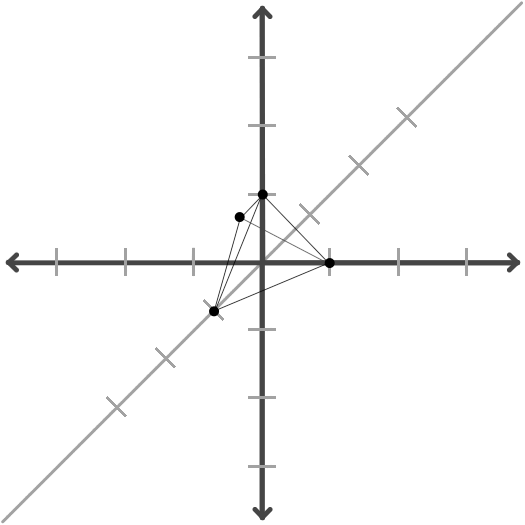
\includegraphics{img/scaling_before-rotation_before.png}
		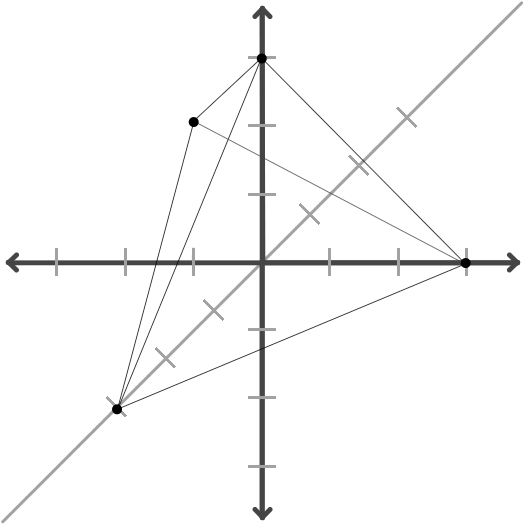
\includegraphics{img/scaling_after.png}
		\caption{Visualization of scaling operation.}
	\end{figure}

	\section{Rotation}

	Rotation translates each point of a figure about an axis, so that the distance of each point from the axis is conserved. Rotation is used extensively in 3D graphics. From simply spinning an object on its axis to draw interest, to rotating the entire environment around the camera to allow for exploration, this is one of the most complex, but also most crucial transformations. Rotation can be thought of as the adding of some $\Delta\theta$ to the built-in angle of a point-vector. Along this logic, the angle addition trig identities can be used: \par
	\[\cos(\theta + \Delta\theta) = \cos(\theta)\cos(\Delta\theta) - \sin(\theta)\sin(\Delta\theta)\]
	\[\sin(\theta + \Delta\theta) = \sin(\theta)\cos(\Delta\theta) + \cos(\theta)\sin(\Delta\theta)\]
	
	The axis that is being rotated about can be thought of as the axis that is coming out of the page. With this visualization, we can see what "cosine" and "sine" mean in the context of this three-dimensional environment: \par

	When rotating about the Z-axis, the axes look identical to a typical set of 2-dimensional axes. The cosine from the central angle will yield the x-component, and the sine will yield the y-component. When rotating about the Y-axis, the Y-axis disappears, and is replaced by the Z-axis. This means that the cosine will still relate to the x-component. However, the sine of the angle will now be related to the z-component of the vector. Finally, when rotating about the X-axis, there are two replacements. The Y-axis moves to the horizontal, and the Z-axis moves to the vertical. This associates that cosine with the y-direction and the sine with the z-direction. \par
		\begin{figure}[H]
			\centering
			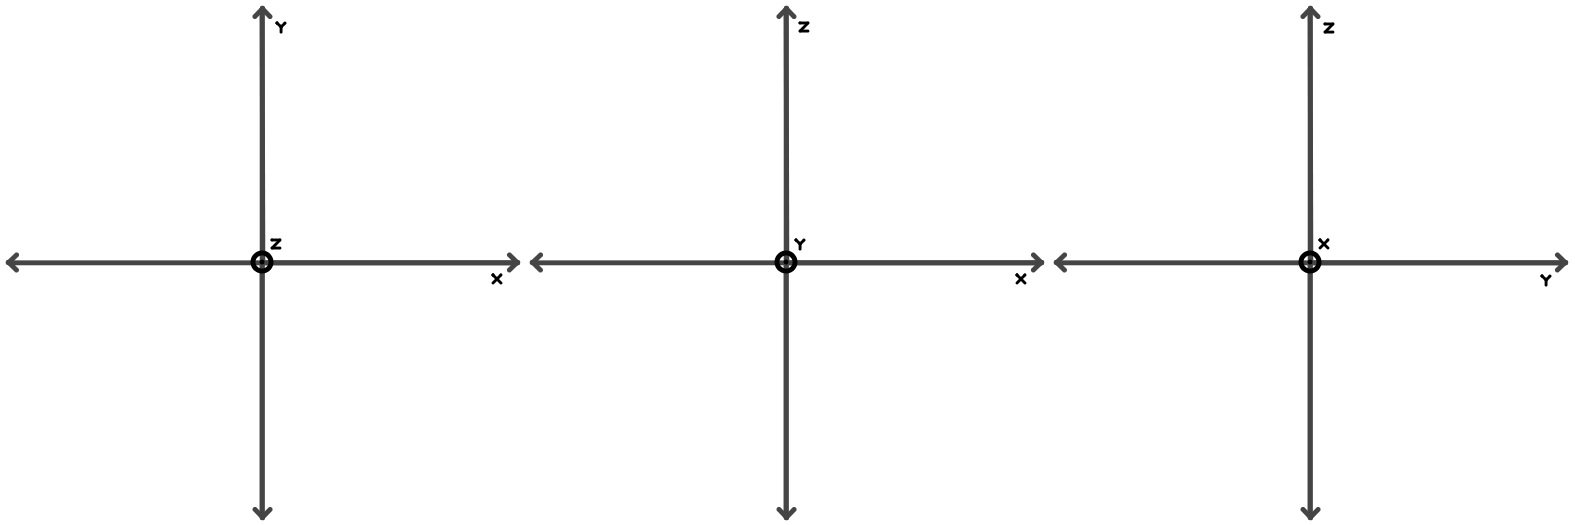
\includegraphics[width=0.85\linewidth]{img/axes.png}
			\caption{The axes to be used for each rotation}
		\end{figure}

	\subsection{Rotation About the Z-axis}

	If rotation is occurring about the Z-axis, then the z-component of the position vector will be conserved. This means that the x and y components of the vector will be the ones changing. For each axis of rotation, the value of cosine and sine in the angle addition trig identity will be replaced with the corresponding value listed in the previous section. For the z-axis, this looks the most familiar to us. The cosine is associated with the x-component of the position vector, and the sine is associated with the y-component. So then, the angle addition formulas could be rewritten in this way:
	\[\cos(\theta + \Delta\theta) = x\cos(\Delta\theta) - y\sin(\Delta\theta)\]
	\[\sin(\theta + \Delta\theta) = x\sin(\Delta\theta) + y\cos(\Delta\theta)\]
	\par
	The top cosine equation will yield the new x-component of the rotated position vector, and the sine equation, the y-component. This means that we want the cosine equation to be on the topmost row of the transformation matrix, and the sine equation in the second row. The third and fourth rows need to stay as they are in the identity matrix in order to preserve the z- and w-components. \par
	In order to get the x and y values in their respective places in the equations above, the result of the matrix multiplication have to be considered. Everything in the left-most column is going to be multiplied by the x-component of the vector, the next column by the y-component, and so on. Using this knowledge, we can construct the following matrix rotation matrix: \par
	\[
		\begin{bmatrix}
			\cos(\Delta\theta) & -\sin(\Delta\theta) & 0 & 0 \\
			\sin(\Delta\theta) &  \cos(\Delta\theta) & 0 & 0 \\
			0 & 0 & 1 & 0 \\
			0 & 0 & 0 & 1
		\end{bmatrix}
	\]

	By multiplying this with a generic position vector, it can be seen that the desired results are achieved by this matrix: \par
	\[
		\begin{bmatrix}
			\cos(\Delta\theta) & -\sin(\Delta\theta) & 0 & 0 \\
			\sin(\Delta\theta) &  \cos(\Delta\theta) & 0 & 0 \\
			0 & 0 & 1 & 0 \\
			0 & 0 & 0 & 1
		\end{bmatrix}
		\bullet
		\begin{pmatrix}
			x \\
			y \\
			z \\
			1
		\end{pmatrix}
		=
		\begin{pmatrix}
			x\cos(\Delta\theta) - y\sin(\Delta\theta) \\
			x\sin(\Delta\theta) + y\cos(\Delta\theta) \\
			z \\
			1
		\end{pmatrix}
	\]

	\subsection{Rotation About the X-axis}

	Rotation about the other two axes is relatively trivial once one axis is understood. The rotation matrix just needs to be edited slightly so that the components that are being affected match the set of axes that were defined at the beginning. \par
	For rotation about the x-axis, the y-axis is the "horizontal," and the z-axis is the "vertical." So, the cosine function is associated with the y-component, and the sine function is associated with the z-component of the position vector. The rotation matrix from the z-axis rotation can be rearranged to pertain to the y- and z-components as follows: \par
	\[
		\begin{bmatrix}
			1 & 0 & 0 & 0 \\
			0 & \cos(\Delta\theta) & -\sin(\Delta\theta) & 0 \\
			0 & \sin(\Delta\theta) &  \cos(\Delta\theta) & 0 \\
			0 & 0 & 0 & 1
		\end{bmatrix}
		\bullet
		\begin{pmatrix}
			x \\
			y \\
			z \\
			1
		\end{pmatrix}
		=
		\begin{pmatrix}
			x \\
			y\cos(\Delta\theta) - z\sin(\Delta\theta) \\
			y\sin(\Delta\theta) + z\cos(\Delta\theta) \\
			1
		\end{pmatrix}
	\]

	\subsection{Rotation About the Y-axis}
	Going through the same process as the x- and z-axes, the following can be found: \par
	\[
		\begin{bmatrix}
			\cos(\Delta\theta) & 0 & -\sin(\Delta\theta) & 0 \\
			0 & 1 & 0 & 0 \\
			\sin(\Delta\theta) & 0 &  \cos(\Delta\theta) & 0 \\
			0 & 0 & 0 & 1
		\end{bmatrix}
		\bullet
		\begin{pmatrix}
			x \\
			y \\
			z \\
			1
		\end{pmatrix}
		=
		\begin{pmatrix}
			x\cos(\Delta\theta) - z\sin(\Delta\theta) \\
			y \\
			x\sin(\Delta\theta) + z\cos(\Delta\theta) \\
			1
		\end{pmatrix}
	\]

	\subsection{Example}
	Consider a pyramid with vertices
	\(p_{1} = \begin{psmallmatrix} 0 \\ 1 \\ 0 \\ 1 \\ \end{psmallmatrix}\)
	\(p_{2} = \begin{psmallmatrix} 0 \\ 0 \\ 1 \\ 1 \\ \end{psmallmatrix}\),
	\(p_{3} = \begin{psmallmatrix} 1 \\ 0 \\ 0 \\ 1 \\ \end{psmallmatrix}\), and
	\(p_{4} = \begin{psmallmatrix} -1 \\ 0 \\ -1 \\ 1 \\ \end{psmallmatrix}\)
	that should be rotated 20 degrees about the y-axis. 
	In order to rotate this figure, the rotation transformation needs to be applied to each point. By substituting 20 degrees into the rotation matrix determined earlier, we can find the resultant points:
	\[
		p'_{1} =
		\begin{bmatrix}
			\cos(20) & 0 & -\sin(20) & 0 \\
			0 & 1 & 0 & 0 \\
			\sin(20) & 0 &  \cos(20) & 0 \\
			0 & 0 & 0 & 1
		\end{bmatrix}
		\bullet
		\begin{pmatrix}
			0 \\ 1 \\ 0 \\ 1 \\
		\end{pmatrix}
		=
		\begin{pmatrix}
			0 \\ 1 \\ 0 \\ 1 \\
		\end{pmatrix}
	\]
	\[
		p'_{2} =
		\begin{bmatrix}
			\cos(20) & 0 & -\sin(20) & 0 \\
			0 & 1 & 0 & 0 \\
			\sin(20) & 0 &  \cos(20) & 0 \\
			0 & 0 & 0 & 1
		\end{bmatrix}
		\bullet
		\begin{pmatrix}
			0 \\ 0 \\ 1 \\ 1 \\
		\end{pmatrix}
		=
		\begin{pmatrix}
			-0.342 \\ 0 \\ 0.940 \\ 1 \\
		\end{pmatrix}
	\]
	\[
		p'_{3} =
		\begin{bmatrix}
			\cos(20) & 0 & -\sin(20) & 0 \\
			0 & 1 & 0 & 0 \\
			\sin(20) & 0 &  \cos(20) & 0 \\
			0 & 0 & 0 & 1
		\end{bmatrix}
		\bullet
		\begin{pmatrix}
			1 \\ 0 \\ 0 \\ 1 \\
		\end{pmatrix}
		=
		\begin{pmatrix}
			0.940 \\ 0 \\ 0.342 \\ 1 \\
		\end{pmatrix}
	\]
	\[
		p'_{4} =
		\begin{bmatrix}
			\cos(20) & 0 & -\sin(20) & 0 \\
			0 & 1 & 0 & 0 \\
			\sin(20) & 0 &  \cos(20) & 0 \\
			0 & 0 & 0 & 1
		\end{bmatrix}
		\bullet
		\begin{pmatrix}
			-1 \\ 0 \\ -1 \\ 1 \\
		\end{pmatrix}
		=
		\begin{pmatrix}
			-0.598 \\ 0 \\ -1.28 \\ 1 \\
		\end{pmatrix}
	\]

	\begin{figure}[H]
		\centering
		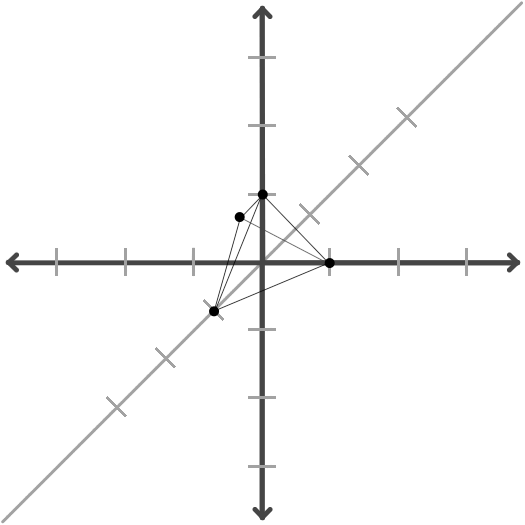
\includegraphics{img/scaling_before-rotation_before.png}
		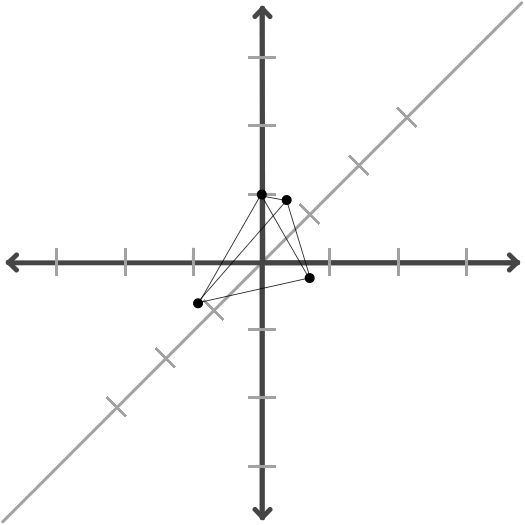
\includegraphics{img/rotation_after.png}
		\caption{Visualization of rotation operation.}
	\end{figure}

	\section{Conclusion}
	3D transformation literally opens up a new dimension to math. Understanding and being able to implement these transformations is the first step in being able to model and simulate the real world around us in new and more complex ways. Throughout this exploration, I have become better acquainted with what is possible using math and computer processing. These concepts are already being implemented extensively by consumer-facing video game companies, and also by scientists and researchers. As computers become more powerful, this math, along with everything that stems off from it, can be implemented to begin to create fully accurate models and representations of our real world. This could be in the form of hyper-realistic computer graphics, increasingly accurate weather models, or even simulating our universe to gain a better understanding of our natural world. \par
	This exploration opened my eyes to the power, and importance, of the matrix. Especially in the context of 3D graphics, the matrix allows for a powerful way to quickly transform several values in a fast and predictable way. In the case of rotations, the transformation matrix allows for the transformation of two different coordinates simultaneously in order to create the rotation. Without a matrix, it would be necessary to operate on each coordinate individually, and so performing a rotation would require two operations instead of one. This is just an example of course, and I suspect that this exploration does not begin to scratch the surface of what matrices are capable of. \par
	I am excited to continue to learn about 3D graphics maths, along with matrices and what they are capable of.

	\newpage

	\section{Works Cited}
	"Translation Transformation," \textit{OGL Dev}. ogldev.atspace.co.uk/www/tutorial06/tutorial06.html. \\
	"Rotation Transformation," \textit{OGL Dev}. ogldev.atspace.co.uk/www/tutorial07/tutorial07.html. \\
	"Scaling Transformation," \textit{OGL Dev}. ogldev.atspace.co.uk/www/tutorial08/tutorial08.html. \\
	"How to Multiply Matrices" \textit{Mathisfun}. https://www.mathsisfun.com/algebra/matrix-multiplying.html.

\end{document}